\documentclass{article}
\usepackage{graphicx} % Required for inserting images
\usepackage{amsmath,amssymb,amsthm}
\usepackage{physics}
\usepackage{graphicx,float}
\graphicspath{{images/}}
\usepackage[none]{hyphenat}
\usepackage{blindtext}
\usepackage{parskip}
\usepackage[letterpaper,top=3cm, left= 3cm,bottom=3cm]{geometry}
\usepackage{subcaption}



\title{Applying Properties of Definite Integrals}
\author{Polaris}
\date{2025/06/23}

\begin{document}

\maketitle

\section{Properties of Definite Integrals}
First Property:
\[
\int_{a}^{b} kf(x)\mathrm{ d}x = k\int_{a}^{b} f(x)\mathrm{ d}x
\]
Where $k$ is any constant, \emph{remember, only constants can be pulled out from the integrand}. For example:
\[
\int_{2}^{4} 4x^2 \mathrm{d}x = 4\int_{2}^{4}x^2 \mathrm{d}x
\]
But 
\[
\int_{2}^{4}4x^2 \mathrm{d}x \neq 4x\int_{2}^{4}x \mathrm{d}x
\]
Since $4x$ is a function of $x$, it is not a constant anymore.

Second property:
\[
\int_{a}^{b} \left(f(x) \pm g(x)\right) \mathrm{d}x = \int_{a}^{b} f(x) \mathrm{d}x \pm \int_{a}^{b} g(x) \mathrm{d}x
\]

This has a nice geometric explanation, on the left, it is a sum of two area, on the right, it is also a sum of two area.

\begin{figure}[H]
    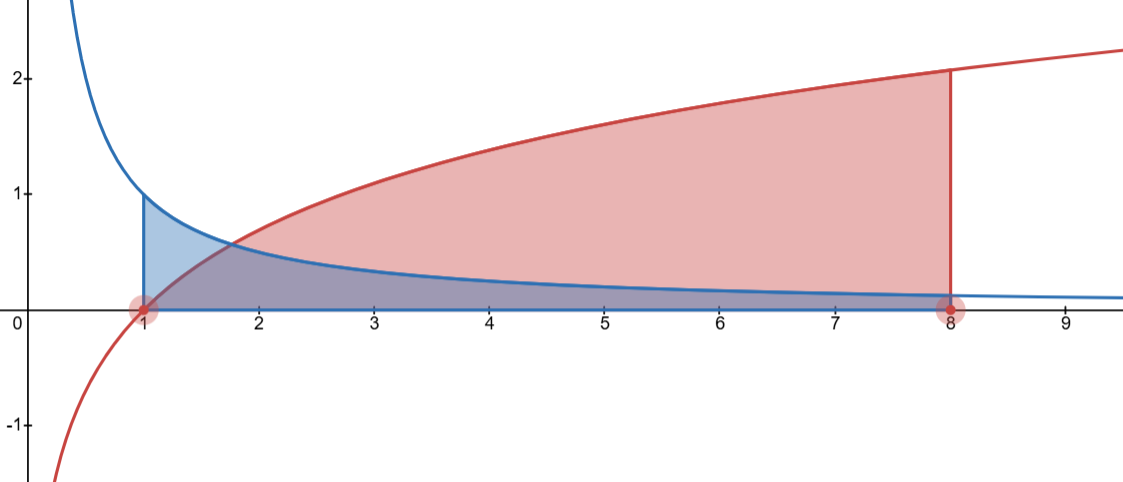
\includegraphics[width = 10cm]{addition.png}
    \centering
    \caption{Graph of $f(x)$ and $g(x)$ and its integral}
\end{figure}

\begin{figure}[H]
    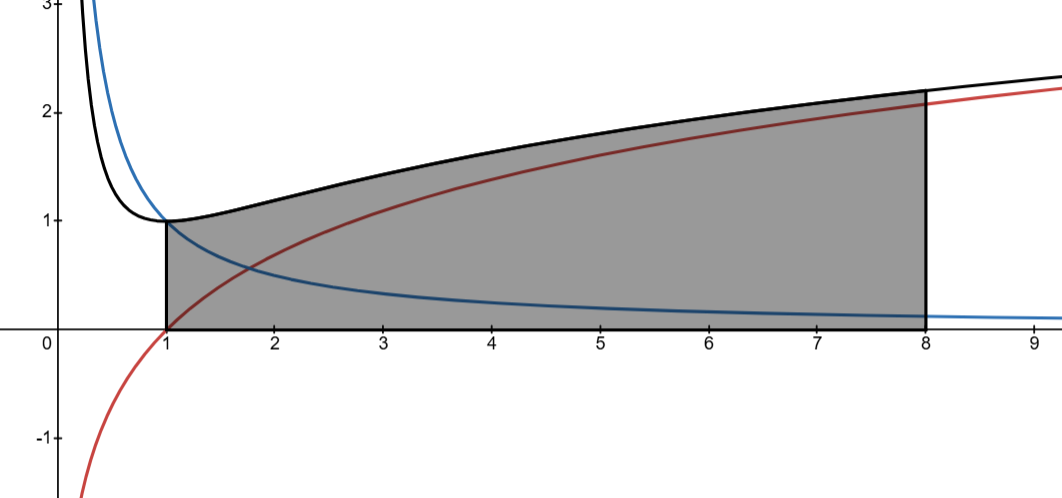
\includegraphics[width = 10cm]{addition2.png}
    \centering
    \caption{Graph of $h(x) = f(x) + g(x)$ and its integral}
\end{figure}

Looking back at Riemann Sum, we know that the area under a curve can be seen as a collection of rectangle, since $h(x) = f(x) + g(x)$,
when computing the Riemann Sum of $h(x)$, its rectangle height is the sum of the height of $f(x)$ and $g(x)$, thus proving this theorem.

A common mistake is assuming that multiplication and division also follows this property, however \emph{this is not true}, in other words:
\[
\int_{a}^{b} f(x)\cdot g(x) \neq \int_{a}^{b} f(x) \cdot \int_{a}^{b}g(x)
\]

Third property:
For the sake of simplifing calculations, we define:
\[
\int_{a}^{b} f(x) \mathrm{d}x = -\int_{b}^{a} f(x) \mathrm{d}x
\]

Fourth property:
Also for the sake of simplifiing calculations, we define:
\[
\int_{a}^{a} f(x) \mathrm{d}x = 0
\]
Which means when the integration bounds are equal, the integrand returns 0.

Fifth property:
\[
\int_{a}^{b} f(x) \mathrm{d}x = \int_{a}^{c} f(x) \mathrm{d}x + \int_{c}^{b} f(x) \mathrm{d}x 
\]
Where $a<b<c$

This one also have a nice geometric explanation
\begin{figure}[H]
    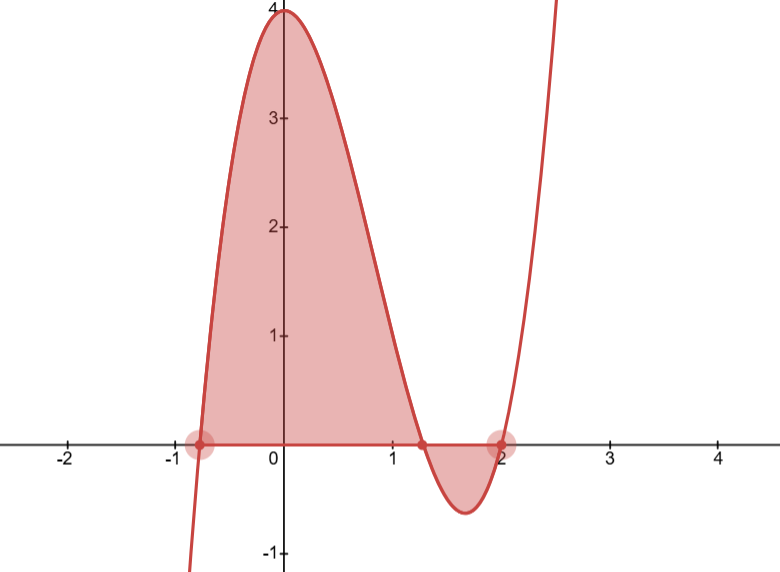
\includegraphics[width = 10cm]{interval.png}
    \centering
    \caption{Graph of $f(x)$}
\end{figure}
The integration bound of this function is denoted as $a$ and $b$, $c$ is the point between them,
to calculate the whole area under the graph, we can first calculate the area under the left half, and then the right half,
translate this to math equations, we have:
\[
\int_{a}^{b} f(x) \mathrm{d}x = \int_{a}^{c} f(x) \mathrm{d}x + \int_{c}^{b} f(x) \mathrm{d}x 
\]

For the sake of simplifying calculations, we define 
\[
\int_{a}^{b} f(x) \mathrm{d}x = \int_{a}^{c} f(x)\mathrm{d}x + \int_{c}^{b} f(x)\mathrm{d}x
\]
No matter what relation $a,b,c$ holds.

\section{Application}
\subsection{Calculating Integral}
Take a look at this example, if 
$\displaystyle \int_{0}^{3} f(x) \mathrm{d}x = 4$, $\displaystyle \int_{0}^{3} g(x) \mathrm{d}x = -1$, find $\displaystyle \int_{0}^{3} \left(5f(x) - 3g(x)\right) \mathrm{d}x$.

To solve this question, we can apply the first and second property of integral:
\begin{align*}
    \int_{0}^{3} \left(5f(x) - 3g(x)\right) \mathrm{d}x &= \int_{0}^{3} 5f(x)\mathrm{d}x - \int_{0}^{3} 3g(x)\mathrm{d}x\\
    &= 5\int_{0}^{3} f(x)\mathrm{d}x - 3\int_{0}^{3}g(x)\mathrm{d}x\\
    &= 5\cdot4 - 3\cdot(-1)\\
    &=23
\end{align*}

Take a look at another example question, if $\displaystyle \int_{-2}^{0} f(x)\mathrm{d}x = 3$, $\displaystyle 4\int_{0}^{3} f(x)\mathrm{d}x = 4$, find $\displaystyle \int_{-2}^{3} 4f(x) \mathrm{d}x$.

To solve this problem, we apply the fifth property of integral and first property of integral:

\begin{align*}
    \int_{-2}^{3} 4f(x)\mathrm{d}x &= 4\left(\int_{-2}^{0} f(x)\mathrm{d}x + \int_{0}^{3} f(x) \mathrm{d}x\right)\\
    &= 4(3+4) = 28
\end{align*}

\subsection{Integrals with discontinuities}
Recall from unit 1, there are 3 types of discontinuities: jump discontinuities, removeable discontinuities and infinite discontinuities. 

We will be discussing integrals related to jump and removable discontinuities.

\subsubsection{Jump Discontinuities}
Consider this function $\displaystyle f(x) = \frac{(x-6)(0.5x+1)}{\abs{x-6}}$, the graph of $f(x)$ is shown
\begin{figure}[H]
    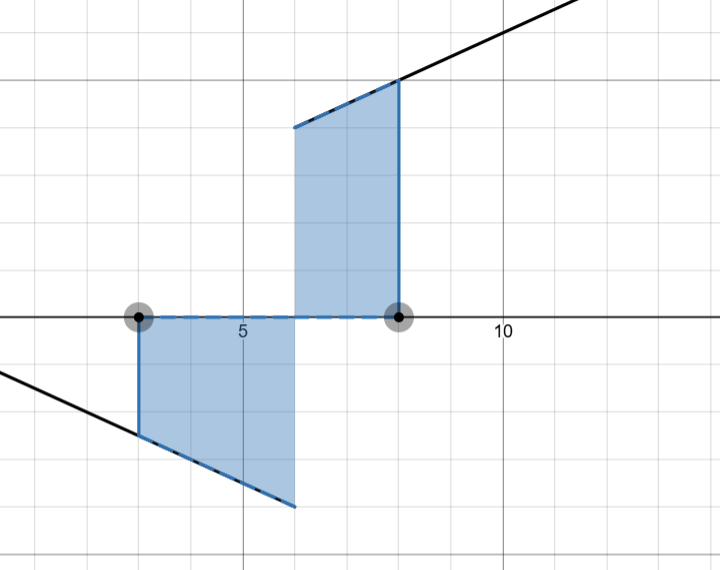
\includegraphics[width=10cm]{jump.png}
    \centering
    \caption{The graph of $f(x)$}
\end{figure}
Find $\displaystyle \int_{3}^{8}f(x)\mathrm{d}x$.

To solve this problem, first notice that $f(x)$ has a jump discontinuities at $x=6$, to find this integral, we are essentially finding the area in blue, thus we have
\[
\int_{3}^{8} f(x)\mathrm{d}x = \int_{3}^{6} f(x)\mathrm{d}x + \int_{6}^{8}f(x) \mathrm{d}x
\]
From the graph we can see that $\displaystyle \int_{3}^{6} f(x)\mathrm{d}x = -\frac{1}{2}*(2.5+4)*3 = -9.75$, $\displaystyle \int_{6}^{8} f(x)\mathrm{d}x = \frac{1}{2} (4+5)*2 = 9$ (hint: area of trapezoid)

The final integral is thus
\[
\int_{3}^{8} f(x)\mathrm{d}x = \int_{3}^{6} f(x)\mathrm{d}x + \int_{6}^{8}f(x) \mathrm{d}x = -9.75 + 9 = -0.75
\]

\subsubsection{Removable Discontinuities}
Consider this function $\displaystyle f(x) = \frac{(2x-1)(x-3)}{(x-3)}$, the graph is shown below.
\begin{figure}[H]
    \centering
    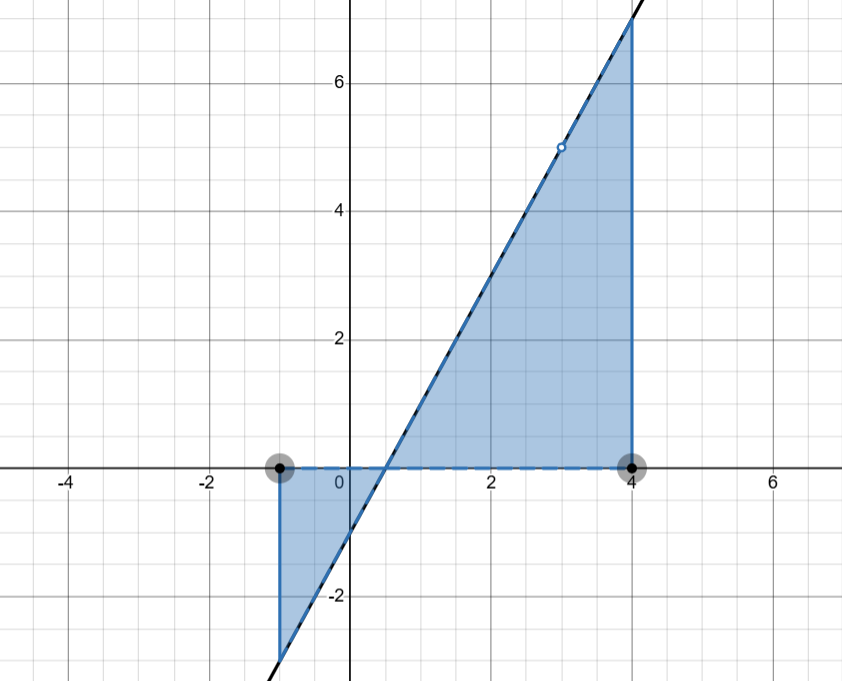
\includegraphics[width=10cm]{remove.png}
    \caption{Graph of $f(x)$}
\end{figure}
Find $\displaystyle \int_{-1}^{4} f(x)\mathrm{d}x$, the area shaded in blue.

Notice that this function has a removable discontinuities at $x=3$, we have:
\[
\int_{-1}^{4} f(x)\mathrm{d}x = \int_{-1}^{3}f(x)\mathrm{d}x + \int_{3}^{4}f(x)\mathrm{d}x
\]
Through geometric observation (computing the area of triangle), the final answer is $\displaystyle \int_{-1}^{4}f(x)\mathrm{d}x = 10$
\end{document}